\chapter*{Proposition 20}
\label{prop:20}

\begin{figure*}[ht]
    \begin{center}
    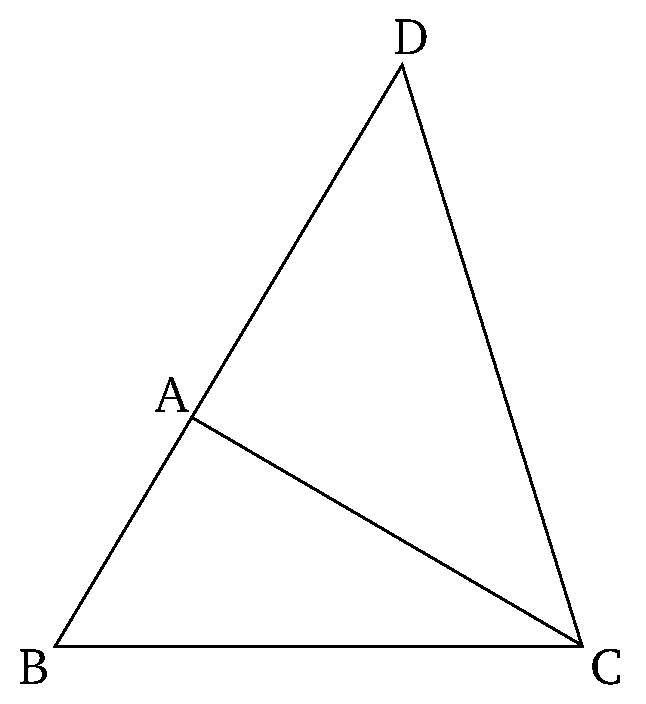
\includegraphics[width=0.5\linewidth]{figures/fig20e.eps}
    \label{fig:prop_20}
    \end{center}
\end{figure*}

In any triangle, (the sum of) two sides taken together in any (possible way) is greater than the remaining (side).

For let $ABC$ be a triangle. I say that in triangle $ABC$ (the sum of) two
sides taken together in
any (possible way) is greater than the remaining (side). (So), (the sum of) $BA$ and $AC$ (is greater) than $BC$,
(the sum of) $AB$ and $BC$ than $AC$, and (the sum of) $BC$ and $CA$ than $AB$.

For let $BA$ have been drawn through to point $D$, and let $AD$ be made equal to $CA$ [Prop.~1.3], and let $DC$ have been joined.

Therefore, since $DA$ is equal to $AC$, the angle $ADC$ is also equal to
$ACD$ [Prop.~1.5]. Thus, $BCD$ is greater than $ADC$. And since
 $DCB$ is a triangle having the angle $BCD$ greater than $BDC$, and the
greater angle subtends the greater side [Prop.~1.19], $DB$ is thus
greater than $BC$. But $DA$ is equal to $AC$. Thus, (the sum of) $BA$ and $AC$ is
greater than $BC$. Similarly, we can show that (the sum of) $AB$ and $BC$ is also
greater than $CA$, and (the sum of) $BC$ and $CA$ than $AB$.

Thus, in any triangle, (the sum of) two sides taken together in any (possible way) is greater than the remaining (side). (Which is) the very thing
it was required to show.


\section*{Commentary}

\begin{proposition}\label{proposition_20}\lean{Elements.Book1.proposition_20}\leanok
    In $\triangle~ABC$, we have $|BA| + |AC|~>~|BC|$.
\end{proposition}
\begin{proof}
    \uses{proposition_3,proposition_5',proposition_19}\leanok
    See the original proof by Euclid.
\end{proof}
